\section{Evaluation}
\label{section-evaluation}

In this section we evaluate our ideas about the debugger that we designed, by answering RQ3. 
The goal of the experiment is to measure the \textit{time} required to solve programming problems~\cite{ko2015practical}. We use time instead of correctness as it matches debugging better: a developer needs to continue debugging \textit{until} he finds an explanation or a solution to his problem. During debugging incorrect assumptions can be tested and corrected. We measure the time from the moment the participant receives the question until the correct answer is given. Participants use either the built-in Chrome Browser debugger (group `Console') or - the treatment - our RxFiddle debugger (group `RxFiddle'). This single alternative debugger together with the experiment UI (which acts as a small IDE) offers all the debugging capabilities subjects of our preliminary interview (RQ1) reported to use.

The experiment consists of a questionnaire, a warm-up task and 4 programming tasks, all available in a single in-browser application. The questionnaire contains questions regarding age, experience in several programming languages and several reactive programming frameworks. We use this self estimation as a measurement of skill instead of a pretest, since it is a faster and better estimator~\cite{kleinschmager2011rate,feigenspan2012measuring,siegmund2014measuring}. The warm-up program is situated in the same environment as the programming problems and contains several tasks designed to let the participants use every control of the test environment. The first 2 programming problems require the participants to obtain an understanding about the behavior of the program and report the findings. The last 2 programming problems contain a program with a bug. The participants are asked to find the event that lead to the bug in the third problem and to identify and propose a solution in the fourth problem. The first 2 problems are synthetic examples of two simple data flows, while the latter contain some mocked (otherwise remote) service which behaves like a real world example.

We use a between-subjects design for our setup. While this complicates the results - subjects have different experience and skills - we can not use a within-subjects design as it would be impossible to control for the learning effect incurred when asking subjects to perform survey questions with and without the tool. This also allows us to restrict the amount of tasks to incorporate in the experiment, requiring less time of our busy subjects.

%\todo{Discuss guidelines defined in ko2015practical~\cite{ko2015practical}}

\subsection{Context}
The experiment was run in a controlled and an online setting.
The controlled experiment was conducted at a Dutch software engineering company. Subjects are developers with several years of programming experience, and range from little to no experience with RP to many years of experience (Figure \ref{fig-experience}). Some of the subjects had already used RxFiddle, forming a potential threat to validity. As we do not try to measure the effect of learning a new tool, but rather using a tool after learning to use it, we explained RxFiddle in the introductory talk and added the warm-up question to get every participant to a minimum amount of knowledge about the debugger at hand.

The online experiment was announced by several core contributors to RP libraries on Twitter and via various other communication channels. Subjects to the online experiment took the test at their own preferred location and have possibly very different backgrounds. Several short video tutorials were created and included in the online experiment to introduce the participants to the debug tool available to them and the tasks they needed to fulfill.

\begin{figure}[h]
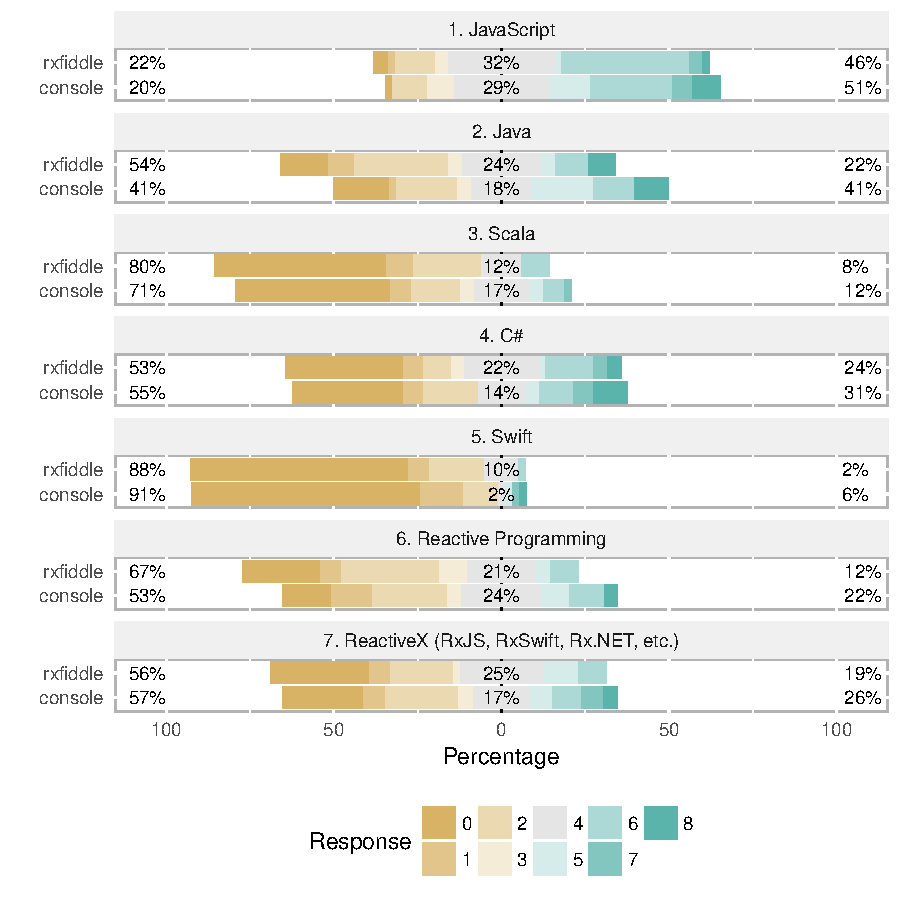
\includegraphics[width=\columnwidth]{images/experience.pdf}
\caption{Experience in various programming languages, 9-point Likert scale}
\label{fig-experience}
\end{figure}

\subsection{Results}
Figure \ref{fig-timePerTask} shows the time until the correct answer was given per task. Here we consider both the results from the controlled experiment as the online experiment, to remedy the small set of subjects available for the controlled experiment. We immediately see some interesting result for task 3. We make no assumptions about the underlying distribution so we perform a non-parametric Wilcoxon Mann-Whitney U test (\textit{$H_0$: times for the Console group and RxFiddle group are drawn from the same population}) to see if the differences are significant, and a Cliffs delta test for ordinal data to determine the effect size.

\begin{centering}
% \begin{table}[]
% \centering
% \caption{My caption}
%\label{my-label}
\begin{tabular}{llllll}
\hline
            & \textbf{$n_1$} & \textbf{$n_2$} & \textbf{W} & \textbf{p-value} & \textbf{Cliffs $\delta$} \\ \hline
\textbf{T1} & 26                      & 30                       & 343        & 0.448           & 0.121     \\
\textbf{T2} & 29                      & 27                       & 362        & 0.637           & 0.0754    \\
\textbf{T3} & 22                      & 24                       & 100        & 0.000186        & 0.621     \\
\textbf{T4} & 15                      & 12                       & 86         & 0.867           & 0.0444    \\ \hline
\end{tabular}
% \end{table}
\end{centering}

For tasks T3 we can reject $H_0$ with high significance ($p < 0.05$), the RxFiddle group is faster.
For the tasks T1, T2 and T4 we can not reject $H_0$ ($p > 0.05$), and for T2 the U test indicates no difference at all, meaning the RxFiddle group and Console group perform or could perform equally.

\begin{figure}[h]
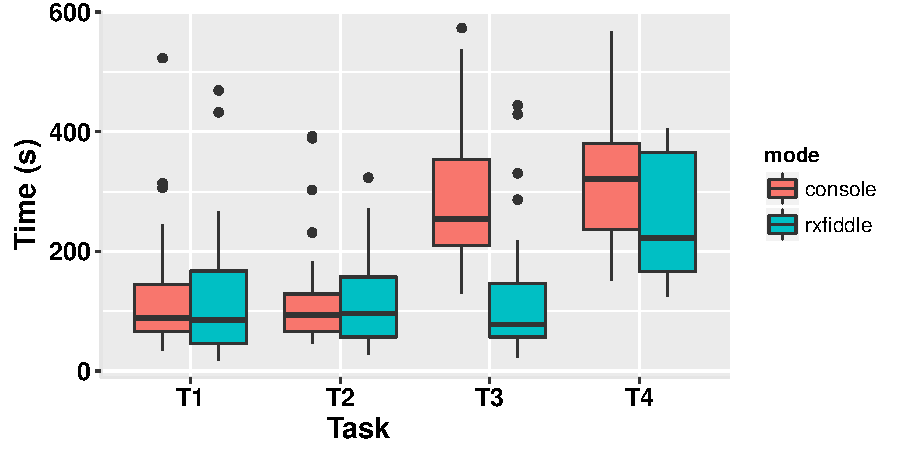
\includegraphics[width=\columnwidth]{images/timePerTask.pdf}
\caption{Time until correct answer per task}
\label{fig-timePerTask}
\end{figure}

While this could be observed as a negative result, RxFiddle is a new tool, and the users have only just been exposed to the tool and received only a short training. More importantly we regarded developers of possibly different experience levels, and developers with more Rx experience might be more familiar with the concepts that RxFiddle visualizes. To investigate this further, we split the results for different groups of subjects, as shown in Figure \ref{fig-timePerTaskSplit}.  When split (at the median value, inclusive) for years of RP experience and the self-assessed RP experience (Likert-scale) we see bigger differences for all tasks for groups with more experience. This indicates that the visualization might be less suitable for inexperienced subjects.

Even while regarding more experienced subjects, the effect is still most significant for T3. We think that RxFiddle might be more suitable to replace traditional debugging for some tasks than others.